\documentclass{standalone}
\usepackage{tikz}
\begin{document}
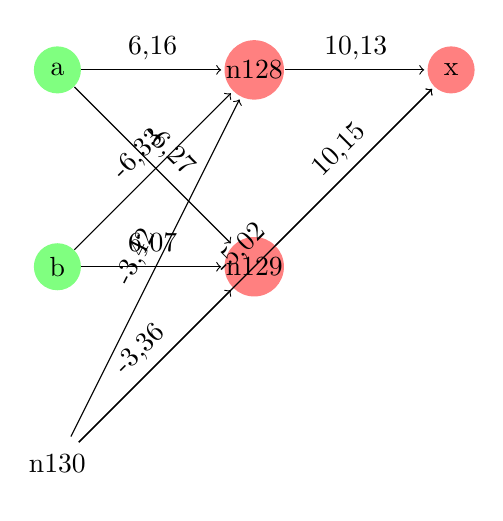
\begin{tikzpicture}[shorten >=1pt,->,draw=black!,node distance=2.5cm]
\tikzstyle{neuron}=[circle,fill=black!25,minimum size=17pt,inner sep=0pt]
\tikzstyle{constant}=[neuron, fill=white!50];
\tikzstyle{sigmoid}=[neuron, fill=red!50];
\tikzstyle{identity}=[neuron, fill=green!50];
\node [identity] (a) {a};
\node [identity,below of=a] (b) {b};
\node [constant,below of=b] (n130) {n130};
\node [sigmoid,right of=a] (n128) {n128};
\node [sigmoid,below of=n128] (n129) {n129};
\node [sigmoid,right of=n128] (x) {x};
\path[every node/.style={sloped,anchor=south,auto=false}]
(n128) edge node {10,13} (x)
(n129) edge node {10,15} (x)
(a) edge node {-6,27} (n129)
(a) edge node {6,16} (n128)
(b) edge node {-6,33} (n128)
(b) edge node {6,07} (n129)
(n130) edge node {-5,02} (x)
(n130) edge node {-3,42} (n128)
(n130) edge node {-3,36} (n129)
;\end{tikzpicture}
\end{document}